\documentclass[12pt,a4paper]{article}

% ---------- Codificación y lengua ----------
\usepackage[utf8]{inputenc}
\usepackage[T1]{fontenc}
\usepackage{lmodern}
\usepackage[spanish,es-nodecimaldot]{babel}

% ---------- Geometría y tipografía ----------
\usepackage[margin=2.5cm]{geometry}
\usepackage{microtype}
\usepackage{amsmath,amssymb,mathtools}
\usepackage{graphicx}
\usepackage{float}
\usepackage{booktabs}
\usepackage{array}
\usepackage{enumitem}
\usepackage[table]{xcolor}
\usepackage[most]{tcolorbox}
\usepackage{caption}
\usepackage[hidelinks]{hyperref}

\linespread{1.04}
\setlength{\parindent}{0pt}
\setlength{\parskip}{0.42em}

\captionsetup[table]{name=Tabla, labelfont=bf, font=small, skip=5pt}
\captionsetup[figure]{labelfont=bf, font=small, skip=5pt}

% ---------- Paleta de las cajas ----------
\definecolor{azulT}{HTML}{466EB4}
\definecolor{azulF}{HTML}{F5F8FF}
\definecolor{grisT}{HTML}{8C8C96}
\definecolor{grisF}{HTML}{F9F9FB}
\definecolor{naranjaT}{HTML}{C88C3C}
\definecolor{naranjaF}{HTML}{FFFAF0}
\definecolor{verdeT}{HTML}{3C8C50}
\definecolor{verdeF}{HTML}{F4FCF5}

\newtcolorbox{cajaIdea}{
  enhanced, colback=azulF, colframe=azulT,
  boxrule=0.6pt, arc=1.5mm, left=7pt, right=7pt, top=4pt, bottom=4pt,
  fontupper=\small
}
\newtcolorbox{cajaVar}{
  enhanced, colback=grisF, colframe=grisT,
  boxrule=0.6pt, arc=1.5mm, left=7pt, right=7pt, top=4pt, bottom=4pt,
  fontupper=\small
}
\newtcolorbox{cajaOjo}{
  enhanced, colback=naranjaF, colframe=naranjaT,
  boxrule=0.6pt, arc=1.5mm, left=7pt, right=7pt, top=4pt, bottom=4pt,
  fontupper=\small
}
\newtcolorbox{cajaRes}{
  enhanced, colback=verdeF, colframe=verdeT,
  boxrule=0.6pt, arc=1.5mm, left=7pt, right=7pt, top=4pt, bottom=4pt,
  fontupper=\small
}

\newcommand{\R}{\mathbb{R}}
\newcommand{\w}{\mathbf{w}}
\newcommand{\x}{\mathbf{x}}
\newcommand{\norm}[1]{\lVert #1\rVert}
\newcommand{\abs}[1]{\lvert #1\rvert}

\graphicspath{{figuras/}}

\begin{document}

% ================= PORTADA =================
\begin{center}
  \vspace*{1.2cm}
  {\Large\bfseries Taller 1 — Teoría de Aprendizaje de Máquina}\\[8pt]
  {\large Clasificación supervisada, vecinos cercanos y evaluación de modelos}\\[6pt]
  {\normalsize Resolución paso a paso, con cálculos manuales y verificación numérica}\\[18pt]
  {\normalsize Juan David Villota}\\[2pt]
  {\small Universidad Nacional de Colombia}\\[2pt]
  {\small 2026-2}
\end{center}

\vspace{0.8cm}
\tableofcontents

\newpage

% ================= CONVENCIONES =================
\section*{Convenciones, notación y símbolos}
\addcontentsline{toc}{section}{Convenciones, notación y símbolos}

Tres convenciones valen para todo el documento. (i) Los vectores son columnas,
de modo que $w^\top x$ es un escalar. (ii) La primera vez que aparece un objeto
se indica su dimensión. (iii) Cada resultado se justifica con la cuenta que lo
produce; no se enuncian fórmulas sin trazabilidad.

\begin{table}[H]
  \centering
  \small
  \caption{Símbolos usados a lo largo del documento.}
  \label{tab:simbolos}
  \begin{tabular}{@{}lll@{}}
    \toprule
    Símbolo & Tipo & Qué es \\
    \midrule
    $x\in\R^2$ & vector columna & observación de entrada \\
    $y\in\{-1,+1\}$ & escalar & etiqueta binaria del perceptrón \\
    $w\in\R^2$, $b\in\R$ & vector, escalar & pesos y sesgo del clasificador lineal \\
    $s(x)=w^\top x+b$ & escalar & puntuación (función afín) \\
    $\hat{y}$ & escalar & clase predicha \\
    $m_i=y_i(w^\top x_i+b)$ & escalar & margen de la observación $i$ \\
    $\eta>0$ & escalar & tasa de aprendizaje del perceptrón \\
    $q$ & vector columna & observación nueva en k-NN \\
    $d(q,x_i)$ & escalar & distancia euclidiana \\
    $k$ & entero & número de vecinos \\
    $TP,TN,FP,FN$ & enteros & celdas de la matriz de confusión \\
    \bottomrule
  \end{tabular}
\end{table}

\begin{cajaVar}
  \textbf{Notación de índices.} En el Problema~1 el subíndice $i$ identifica la
  observación que se está corrigiendo. En el Problema~2, $x_i$ recorre el
  conjunto de entrenamiento y $q$ es el punto que se clasifica. En el
  Problema~3 no hay índices: se cuenta sobre diez pares
  $(y_j,\hat{y}_j)$, $j=1,\dots,10$.
\end{cajaVar}

% ================= PROBLEMA 1 =================
\section{Clasificación lineal y algoritmo del perceptrón}

El perceptrón es el clasificador lineal más simple: busca un hiperplano que
separe las clases y predice según el lado en que cae cada observación. En
$\R^2$ ese hiperplano es una recta. Esta sección resuelve su geometría (1.1),
demuestra la identidad central de la regla de aprendizaje (1.2) y ejecuta un
paso numérico (1.3).

\subsection{Frontera de decisión}

La predicción depende solo del signo de la puntuación
\begin{equation}
  s(x)=w^\top x+b,
  \qquad
  \hat{y}=
  \begin{cases}
    +1, & s(x)>0,\\
    -1, & s(x)\leq 0.
  \end{cases}
  \label{eq:regla}
\end{equation}

Con $w=(1,2)^\top$ y $b=-3$, la frontera $w^\top x+b=0$ es
\begin{equation}
  x_1+2x_2-3=0
  \quad\Longleftrightarrow\quad
  x_2=\frac{3-x_1}{2}.
  \label{eq:frontera}
\end{equation}
Es una recta de pendiente $-1/2$ que corta el eje $x_1$ en $(3,0)$ y el eje
$x_2$ en $(0,3/2)$. El vector $w=(1,2)$ es normal a la recta y apunta hacia el
semiplano donde $s(x)>0$, es decir, hacia la clase $+1$. La distancia
euclidiana de un punto a la recta es $\abs{s(x)}/\norm{w}$, con
$\norm{w}=\sqrt{5}$.

\begin{table}[H]
  \centering
  \small
  \caption{Predicción y distancia a la frontera para los cuatro puntos.}
  \label{tab:p11}
  \begin{tabular}{@{}cccccl@{}}
    \toprule
    Punto & $s(x)=x_1+2x_2-3$ & $\hat{y}$ & $y$ & $\abs{s}/\norm{w}$ & Justificación \\
    \midrule
    $x_1=(0,0)$ & $-3$ & $-1$ & $-1$ & $3/\sqrt{5}\approx1.342$ & $s\leq0\Rightarrow-1$ \\
    $x_2=(1,0)$ & $-2$ & $-1$ & $-1$ & $2/\sqrt{5}\approx0.894$ & $s\leq0\Rightarrow-1$ \\
    $x_3=(2,1)$ & $1$  & $+1$ & $+1$ & $1/\sqrt{5}\approx0.447$ & $s>0\Rightarrow+1$ \\
    $x_4=(3,1)$ & $2$  & $+1$ & $+1$ & $2/\sqrt{5}\approx0.894$ & $s>0\Rightarrow+1$ \\
    \bottomrule
  \end{tabular}
\end{table}

La Tabla~\ref{tab:p11} recoge el cálculo punto a punto. Los cuatro puntos
quedan estrictamente fuera de la frontera, así que la regla
no depende de convenciones en el borde. Los márgenes
$m_i=y_i\,s(x_i)$ valen $3$, $2$, $1$ y $2$: todos positivos, de modo que la
predicción coincide con la etiqueta en los cuatro casos. El punto positivo más
cercano a la recta es $x_3=(2,1)$, a $1/\sqrt{5}\approx0.447$ unidades; el más
alejado es $x_1=(0,0)$, a $3/\sqrt{5}\approx1.342$. Esa cercanía importa: un
cambio pequeño de $w$ o $b$ puede mover la frontera y cambiar la clase de
$x_3$ antes que la de los demás. La Figura~\ref{fig:frontera} resume la
situación.

\begin{cajaOjo}
  \textbf{Detalle que suele confundir.} El signo de $b$ no indica el lado de la
  recta: lo que decide es el signo de $s(x)$. Con $b=-3$ la recta se desplaza,
  pero el semiplano positivo sigue siendo el que está ``a favor'' de $w$. Y la
  distancia es $\abs{s}/\norm{w}$, no $\abs{s}$: dividir por $\norm{w}$ es lo que
  convierte la puntuación en una longitud.
\end{cajaOjo}

\begin{figure}[htbp]
  \centering
  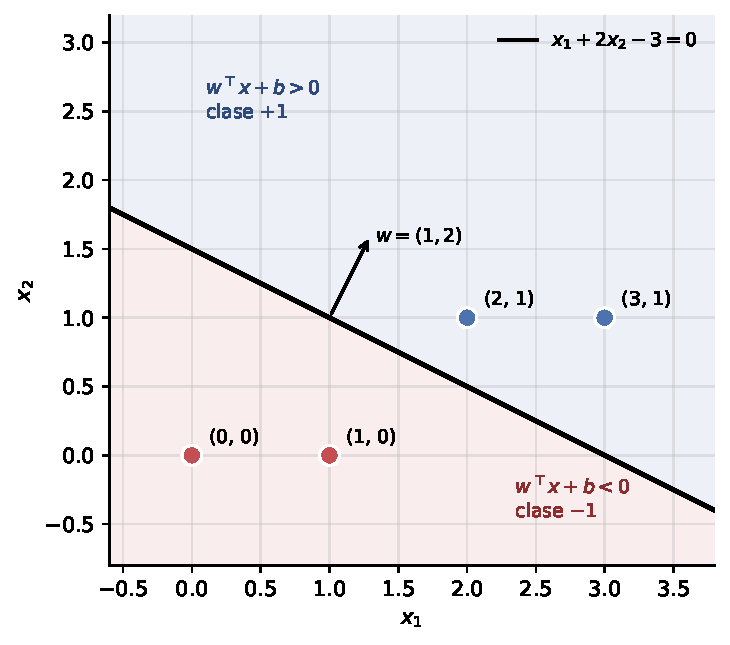
\includegraphics[width=0.72\textwidth]{p1_frontera.pdf}
  \caption{Frontera $x_1+2x_2-3=0$. La zona azul es la región $+1$ y la roja la
  región $-1$. La flecha es el vector normal $w=(1,2)$, que apunta hacia el lado
  positivo. Los puntos se colorean según su etiqueta verdadera.}
  \label{fig:frontera}
\end{figure}

\subsection{Actualización del perceptrón}

Cuando una observación $(x_i,y_i)$ está mal clasificada se aplica
\begin{equation}
  w_{\text{nuevo}}=w+\eta\,y_i x_i,
  \qquad
  b_{\text{nuevo}}=b+\eta\,y_i,
  \qquad \eta>0.
  \label{eq:update}
\end{equation}
El margen de esa observación es $m_i=y_i\,(w^\top x_i+b)$. Antes de actualizar,
$m_i>0$ significa clasificación correcta, $m_i=0$ que el punto está en la
frontera y $m_i<0$ clasificación incorrecta.

\begin{cajaIdea}
  \textbf{Qué se quiere demostrar.} Que inmediatamente después de la
  actualización, y para la misma observación,
  \begin{equation}
    m_{i,\text{nuevo}}=m_i+\eta\bigl(\norm{x_i}_2^2+1\bigr).
    \label{eq:margen}
  \end{equation}
\end{cajaIdea}

\textbf{Demostración.} Se sustituye \eqref{eq:update} en la definición del
margen y se usa $y_i^2=1$:
\begin{equation}
\begin{aligned}
  m_{i,\text{nuevo}}
  &= y_i\bigl(w_{\text{nuevo}}^\top x_i+b_{\text{nuevo}}\bigr)\\
  &= y_i\bigl((w+\eta y_i x_i)^\top x_i+b+\eta y_i\bigr)\\
  &= y_i\bigl(w^\top x_i+b\bigr)
     +\eta\,y_i^2\,x_i^\top x_i
     +\eta\,y_i^2\\
  &= m_i+\eta\,\norm{x_i}_2^2+\eta\\
  &= m_i+\eta\bigl(\norm{x_i}_2^2+1\bigr).
\end{aligned}
  \label{eq:demo}
\end{equation}
En el tercer paso se distribuyó el producto y se usó que
$(y_i x_i)^\top x_i=y_i\,x_i^\top x_i$; en el cuarto, $y_i^2=1$ y
$x_i^\top x_i=\norm{x_i}_2^2$.

\textbf{Qué implica el resultado.}

\begin{enumerate}[leftmargin=1.4em,itemsep=0.25em]
  \item El margen de la observación corregida \emph{siempre aumenta}, en la
  cantidad estrictamente positiva $\eta(\norm{x_i}^2+1)$. El aumento no depende
  de $w$, de $b$ ni del valor actual del margen.
  \item El aumento crece con $\norm{x_i}^2$: observaciones con norma
  grande reciben una corrección mayor. Por eso, si las variables tienen escalas
  muy distintas, conviene normalizarlas antes de entrenar.
  \item Aumentar el margen \emph{no garantiza} que la observación quede bien
  clasificada en un solo paso. Si $m_i<-\eta(\norm{x_i}^2+1)$, el nuevo margen
  sigue siendo negativo. Por ejemplo, con $\eta=0.1$, $x_i=(1,0)$ y $m_i=-1$,
  el nuevo margen es $-1+0.1(1+1)=-0.8<0$.
  \item La identidad es local: describe el efecto sobre la observación que
  disparó la actualización. Otros puntos pueden empeorar su margen con el mismo
  cambio de $w$ y $b$. Por eso el perceptrón no minimiza una función objetivo
  global y su convergencia se estudia aparte (teorema de Novikoff para datos
  separables).
\end{enumerate}

\begin{cajaOjo}
  \textbf{Detalle que suele confundir.} El margen no salta a un valor fijo:
  aumenta en una cantidad fija. Y el resultado habla del margen de \emph{esa}
  observación, no del margen mínimo del conjunto ni del número de errores.
\end{cajaOjo}

\subsection{Ejercicio numérico}

Con $w=(0,0)^\top$, $b=0$, $\eta=0.5$, $x=(2,1)^\top$ y $y=+1$, la puntuación
inicial es
\begin{equation}
  s(x)=w^\top x+b=0\cdot2+0\cdot1+0=0.
\end{equation}
Como la regla \eqref{eq:regla} asigna $+1$ solo cuando $s(x)>0$, la predicción
es $\hat{y}=-1$, distinta de la etiqueta $y=+1$. La observación está mal
clasificada (en la frontera), así que \textbf{sí corresponde actualizar}:
\begin{equation}
  w_{\text{nuevo}}=(0,0)+0.5\cdot1\cdot(2,1)=(1,\,0.5),
  \qquad
  b_{\text{nuevo}}=0+0.5\cdot1=0.5.
\end{equation}
El margen antes de actualizar era $m=y\,s(x)=0$. Después,
\begin{equation}
  m_{\text{nuevo}}
  =1\cdot\bigl(1\cdot2+0.5\cdot1+0.5\bigr)
  =3,
\end{equation}
y la identidad \eqref{eq:margen} predice
\begin{equation}
  m+\eta\bigl(\norm{x}_2^2+1\bigr)
  =0+0.5\,(2^2+1^2+1)
  =0.5\cdot6=3,
\end{equation}
que coincide. Además, la nueva puntuación es $s_{\text{nuevo}}=3>0$, así que la
observación queda ahora bien clasificada como $+1$. El sesgo pasó de $0$ a
$0.5$: la actualización también desplaza la frontera.

\begin{cajaRes}
  \textbf{Resultado.} $w_{\text{nuevo}}=(1,0.5)$, $b_{\text{nuevo}}=0.5$ y el
  margen pasa de $0$ a $3=0.5(\norm{x}^2+1)$. El paso corrige la observación y
  la deja con margen positivo.
\end{cajaRes}

% ================= PROBLEMA 2 =================
\section{Clasificación por los \texorpdfstring{$k$}{k} vecinos más cercanos}

k-NN es un método no paramétrico basado en instancias: no estima coeficientes,
guarda el conjunto de entrenamiento y decide la clase de una observación nueva
por votación mayoritaria entre sus $k$ vecinos más cercanos. La frontera de
decisión resulta de unir las regiones de Voronoi de los puntos de entrenamiento,
de modo que puede ser arbitrariamente irregular. Su comportamiento depende de
dos elecciones: la distancia y el número de vecinos $k$.

\subsection{Cálculo manual}

La observación nueva es $q=(1,1)$ y el conjunto de entrenamiento es el de la
Tabla~\ref{tab:knn}. Se usa la distancia euclidiana
\begin{equation}
  d(q,x_i)=\sqrt{(q_1-x_{i,1})^2+(q_2-x_{i,2})^2}.
  \label{eq:dist}
\end{equation}

\begin{table}[H]
  \centering
  \small
  \caption{Conjunto de entrenamiento del enunciado.}
  \label{tab:knn}
  \begin{tabular}{@{}lccccc@{}}
    \toprule
    Observación & $x_1$ & $x_2$ & $x_3$ & $x_4$ & $x_5$ \\
    \midrule
    $x_i$  & $(0,0)$ & $(1,0)$ & $(3,1)$ & $(0,3)$ & $(1.1,1.1)$ \\
    Clase  & A & A & B & B & B \\
    \bottomrule
  \end{tabular}
\end{table}

\begin{table}[H]
  \centering
  \small
  \caption{Distancias a $q=(1,1)$, valor exacto, valor decimal y orden.}
  \label{tab:distancias}
  \begin{tabular}{@{}lcccc@{}}
    \toprule
    $x_i$ & Cálculo & $d(q,x_i)$ exacta & Decimal & Orden \\
    \midrule
    $x_1=(0,0)$     & $\sqrt{1^2+1^2}$   & $\sqrt{2}$        & $1.4142$ & 3 \\
    $x_2=(1,0)$     & $\sqrt{0^2+1^2}$   & $1$               & $1.0000$ & 2 \\
    $x_3=(3,1)$     & $\sqrt{2^2+0^2}$   & $2$               & $2.0000$ & 4 \\
    $x_4=(0,3)$     & $\sqrt{1^2+2^2}$   & $\sqrt{5}$        & $2.2361$ & 5 \\
    $x_5=(1.1,1.1)$ & $\sqrt{0.1^2+0.1^2}$ & $\sqrt{0.02}=\frac{\sqrt{2}}{10}$ & $0.1414$ & 1 \\
    \bottomrule
  \end{tabular}
\end{table}

El orden de cercanía es
\begin{equation}
  x_5 \prec x_2 \prec x_1 \prec x_3 \prec x_4,
\end{equation}
con distancias $0.1414$, $1$, $1.4142$, $2$ y $2.2361$. La votación para cada
$k$ se resume en la Tabla~\ref{tab:votos}.

\begin{table}[H]
  \centering
  \small
  \caption{Vecindad y votación mayoritaria para $k=1,3,5$.}
  \label{tab:votos}
  \begin{tabular}{@{}clcccc@{}}
    \toprule
    $k$ & Vecinos (en orden) & Clases & Votos A & Votos B & Predicción \\
    \midrule
    1 & $x_5$                 & B             & 0 & 1 & B \\
    3 & $x_5,x_2,x_1$         & B, A, A       & 2 & 1 & A \\
    5 & $x_5,x_2,x_1,x_3,x_4$ & B, A, A, B, B & 2 & 3 & B \\
    \bottomrule
  \end{tabular}
\end{table}

\textbf{Por qué $k$ cambia la predicción.} El valor de $k$ fija el radio del
vecindario y, con él, qué parte del conjunto participa en el voto. Para $k=1$
solo cuenta $x_5$, que es de clase B y está a $0.141$ de $q$: la predicción es
local y muy sensible al ruido. Para $k=3$ entran $x_2$ y $x_1$, ambos de clase
A, y la mayoría cambia a A. Para $k=5$ entran $x_3$ y $x_4$, de clase B, y la
mayoría vuelve a B. No hay empates porque $k$ es impar en los tres casos.

\begin{cajaOjo}
  \textbf{Detalle que suele confundir.} La etiqueta de $q$ no es ``la del punto
  más cercano'' salvo cuando $k=1$. Con $k>1$ manda la composición del
  vecindario, y esa composición cambia con el radio. Un $k$ par puede producir
  empate; aquí se evita usando $k$ impar.
\end{cajaOjo}

\subsection{Implementación con \texttt{make\_moons}}

Se generan $N=300$ observaciones bidimensionales con \texttt{make\_moons}
(\texttt{n\_samples=300}, \texttt{noise=0.20}, \texttt{random\_state=42}). La
partición es 70\,\% entrenamiento y 30\,\% prueba, estratificada por clase y con
semilla fija. El resultado son 210 observaciones de entrenamiento (105 por
clase) y 90 de prueba (45 por clase). La Tabla~\ref{tab:acc} resume las
exactitudes y la Figura~\ref{fig:datos} muestra los datos.

\begin{table}[H]
  \centering
  \small
  \caption{Exactitud de k-NN para tres valores de $k$.}
  \label{tab:acc}
  \begin{tabular}{@{}ccccc@{}}
    \toprule
    $k$ & Aciertos train & Exactitud train & Aciertos test & Exactitud test \\
    \midrule
    1  & 210/210 & $1.0000$ & 84/90 & $0.9333$ \\
    5  & 201/210 & $0.9571$ & 86/90 & $0.9556$ \\
    15 & 201/210 & $0.9571$ & 84/90 & $0.9333$ \\
    \bottomrule
  \end{tabular}
\end{table}

\begin{figure}[H]
  \centering
  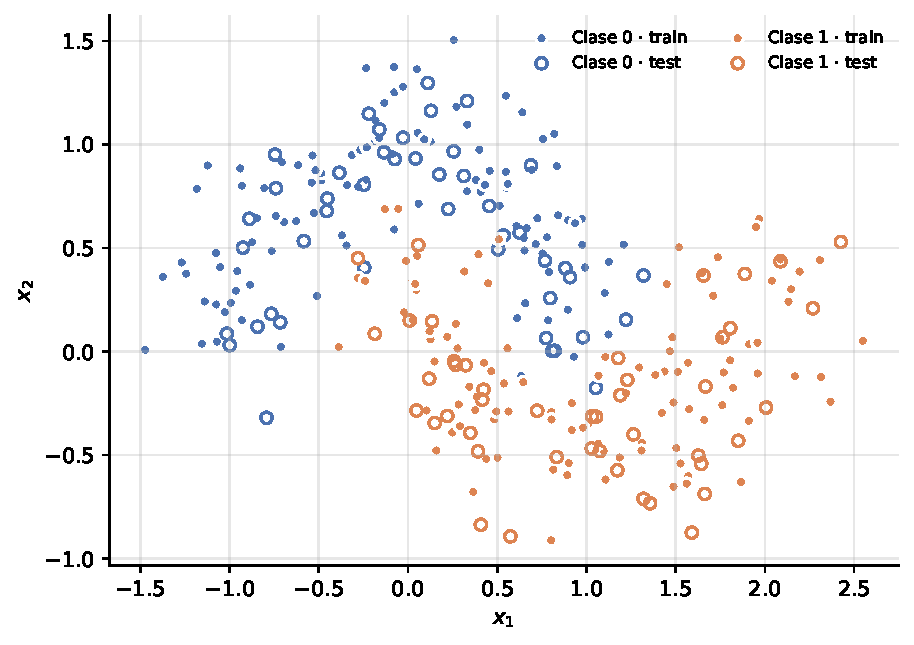
\includegraphics[width=0.72\textwidth]{p2_datos.pdf}
  \caption{Datos de \texttt{make\_moons} con \texttt{noise=0.20}. Puntos
  rellenos: entrenamiento; huecos: prueba. El ruido hace que las dos lunas se
  solapen, de modo que una frontera simple no las separa; $k=1$ solo logra
  separarlas memorizando el entrenamiento.}
  \label{fig:datos}
\end{figure}

\begin{figure}[htbp]
  \centering
  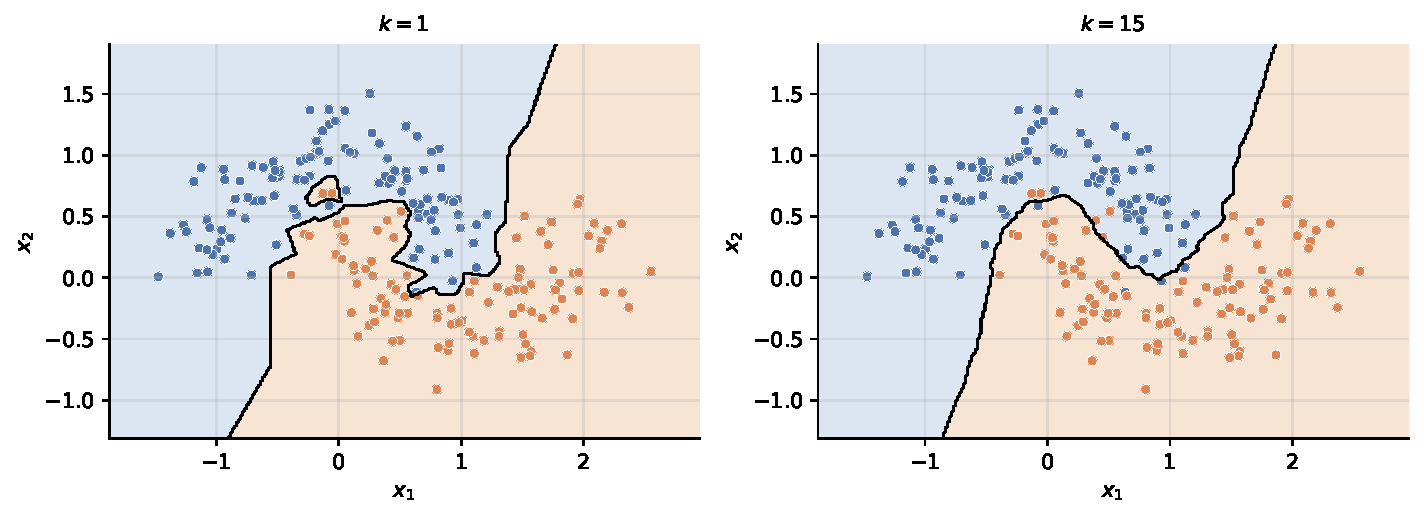
\includegraphics[width=\textwidth]{p2_regiones.pdf}
  \caption{Regiones de decisión con los datos de entrenamiento superpuestos.
  Izquierda: $k=1$, frontera quebrada con islas locales. Derecha: $k=15$,
  frontera más regular que promedia un vecindario amplio.}
  \label{fig:regiones}
\end{figure}

\begin{cajaVar}
  \textbf{Qué mirar en las figuras.} La Figura~\ref{fig:regiones} compara las
  dos fronteras. En $k=1$ la frontera rodea puntos
  individuales y aparecen islas: es la firma de la memorización. En $k=15$ la
  frontera corta las lunas con una curva continua, pero ya incluye puntos de la
  luna contraria cuando el vecindario cruza el solapamiento central.
\end{cajaVar}

\subsection{Interpretación}

\textbf{$k$ muy pequeño.} Con $k=1$ el vecindario es un solo punto: el modelo
reproduce exactamente el conjunto de entrenamiento y alcanza exactitud
$1.0000$ en train. En prueba cae a $0.9333$ (6 errores de 90). La frontera es
irregular y muy sensible al ruido; es el régimen de alta varianza y bajo sesgo.

\textbf{$k$ muy grande.} Con $k=15$ el vecindario abarca una zona amplia. La
frontera se suaviza y la exactitud de train baja a $0.9571$, señal de que el
modelo ya no memoriza. En prueba obtiene $0.9333$: el sesgo aumentó y el
vecindario empieza a mezclar puntos de la otra luna. Es el régimen de baja
varianza y alto sesgo.

\textbf{Mejor compromiso en esta partición.} $k=5$ logra $0.9571$ en train y
$0.9556$ en prueba (4 errores de 90), la mejor exactitud de prueba de las tres.
El vecindario es suficientemente local para seguir la forma de las lunas y
suficientemente amplio para no copiar el ruido.

\textbf{¿Qué tan sólida es la conclusión?} El conjunto de prueba tiene 90
observaciones. Un solo error mueve la exactitud en $1/90\approx1.11$ puntos
porcentuales, y el error estándar de una exactitud cercana a $0.94$ es
$\sqrt{0.94\cdot0.06/90}\approx0.025$, es decir, unos $2.5$ puntos. La
diferencia entre $0.9333$ y $0.9556$ es de dos observaciones: está dentro del
ruido muestral. Se puede afirmar que $k=5$ fue el mejor \emph{en esta
partición}, no que sea el mejor $k$ del problema.

\textbf{Selección formal de $k$.} Elegir $k$ mirando la exactitud de prueba
contamina la evaluación: la prueba deja de ser una estimación independiente y
su valor se vuelve optimista. El procedimiento correcto es seleccionar $k$ con
validación sobre el entrenamiento (por ejemplo, validación cruzada
estratificada de 5 pliegues), quedarse con el $k$ de mejor exactitud media de
validación y usar el conjunto de prueba una sola vez, al final, para reportar
la generalización. Con $N=300$ la validación cruzada además aprovecha mejor los
datos que una única partición.

% ================= PROBLEMA 3 =================
\section{Evaluación de un clasificador binario}

Se tienen diez etiquetas verdaderas y las predicciones del enunciado, con la
clase $1$ como positiva:
\begin{equation}
  y=[0,0,0,0,1,1,1,1,1,1],
  \qquad
  \hat{y}=[0,1,0,0,1,0,1,1,0,1].
\end{equation}

\subsection{Matriz de confusión}

La matriz se construye con las clases reales en las filas y las predichas en
las columnas, en el orden $(0,1)$. Cada celda cuenta pares $(y_j,\hat{y}_j)$:
\begin{itemize}[leftmargin=1.4em,itemsep=0.15em]
  \item $TP$: real $1$ y predicho $1$ (acierto positivo).
  \item $TN$: real $0$ y predicho $0$ (acierto negativo).
  \item $FP$: real $0$ y predicho $1$ (falsa alarma).
  \item $FN$: real $1$ y predicho $0$ (positivo no detectado).
\end{itemize}

Al recorrer los diez pares, los únicos desacuerdos son la posición 2
($y=0$, $\hat{y}=1$, un $FP$) y las posiciones 6 y 9 ($y=1$, $\hat{y}=0$, dos
$FN$). Por tanto
\begin{equation}
  TP=4,\qquad TN=3,\qquad FP=1,\qquad FN=2,
\end{equation}
y la matriz es
\begin{equation}
  C=
  \begin{pmatrix}
    TN & FP\\
    FN & TP
  \end{pmatrix}
  =
  \begin{pmatrix}
    3 & 1\\
    2 & 4
  \end{pmatrix}.
  \label{eq:matriz}
\end{equation}
Las filas suman $4$ (clase real $0$) y $6$ (clase real $1$); las columnas suman
$5$ y $5$. El total es $10=TP+TN+FP+FN$. La Figura~\ref{fig:matriz} representa
la matriz.

\begin{figure}[H]
  \centering
  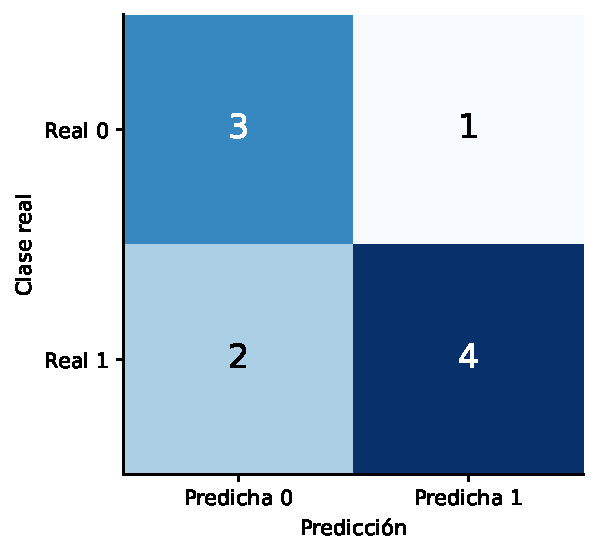
\includegraphics[width=0.60\textwidth]{p3_matriz.pdf}
  \caption{Matriz de confusión del clasificador. La diagonal contiene los
  aciertos ($3+4=7$); fuera de ella quedan una falsa alarma y dos positivos no
  detectados.}
  \label{fig:matriz}
\end{figure}

\subsection{Métricas}

Con los conteos anteriores se calculan las cuatro medidas:
\begin{align}
  \text{Accuracy}
  &=\frac{TP+TN}{TP+TN+FP+FN}
  =\frac{4+3}{10}
  =\frac{7}{10}=0.7000,\\[2pt]
  \text{Precision}
  &=\frac{TP}{TP+FP}
  =\frac{4}{4+1}
  =\frac{4}{5}=0.8000,\\[2pt]
  \text{Recall}
  &=\frac{TP}{TP+FN}
  =\frac{4}{4+2}
  =\frac{4}{6}=\frac{2}{3}\approx0.6667,\\[2pt]
  F_1
  &=\frac{2\,\text{Precision}\cdot\text{Recall}}
          {\text{Precision}+\text{Recall}}
  =\frac{2\cdot\frac45\cdot\frac23}{\frac45+\frac23}
  =\frac{16/15}{22/15}
  =\frac{8}{11}\approx0.7273.
\end{align}

\textbf{Qué evalúa cada medida.}
\begin{itemize}[leftmargin=1.4em,itemsep=0.2em]
  \item \textbf{Exactitud:} proporción total de aciertos. Es simétrica entre
  clases y trata igual un $FP$ y un $FN$.
  \item \textbf{Precisión:} de las observaciones que el modelo marca como
  positivas, qué fracción lo es realmente. Mide la confiabilidad de la alarma
  positiva.
  \item \textbf{Recall:} de los positivos reales, qué fracción se detecta. Mide
  la cobertura; su complemento $1-\text{Recall}=FN/(TP+FN)=1/3$ es la tasa de
  positivos perdidos.
  \item \textbf{$F_1$:} media armónica de precisión y recall. Penaliza los
  desbalances entre ambas; es alta solo si las dos son altas.
\end{itemize}

\textbf{Lectura del caso.} El clasificador es más preciso que sensible: cuando
dice $1$ acierta el $80$\,\% de las veces, pero deja pasar $1/3$ de los
positivos reales. Reportar solo $0.70$ de exactitud oculta esa asimetría.

\subsection{Verificación y análisis}

La Tabla~\ref{tab:verif} compara el cálculo manual con las funciones de
scikit-learn. Los cuatro valores coinciden hasta el cuarto decimal.

\begin{table}[H]
  \centering
  \small
  \caption{Verificación de las métricas con scikit-learn.}
  \label{tab:verif}
  \begin{tabular}{@{}lccc@{}}
    \toprule
    Métrica & Cálculo manual & \texttt{sklearn} & Coincide \\
    \midrule
    Accuracy  & $7/10=0.7000$  & $0.7000$ & Sí \\
    Precision & $4/5=0.8000$   & $0.8000$ & Sí \\
    Recall    & $4/6=0.6667$   & $0.6667$ & Sí \\
    $F_1$     & $8/11=0.7273$  & $0.7273$ & Sí \\
    \bottomrule
  \end{tabular}
\end{table}

\textbf{Dos situaciones en las que la exactitud sola engaña.}

\begin{enumerate}[leftmargin=1.4em,itemsep=0.35em]
  \item \textbf{Clases desbalanceadas.} Supóngase un conjunto con 95 casos
  negativos y 5 positivos. Un clasificador que siempre predice $0$ acierta
  $95/100=0.95$, pero su recall es $0$: no detecta ningún positivo y su
  precisión es indefinida ($0/0$). La exactitud se ve excelente porque la clase
  mayoritaria domina el promedio; las métricas por clase y la matriz de
  confusión revelan el fracaso. Algo análogo ocurre aquí: la clase mayoritaria
  es $1$ ($6/10$), así que el clasificador trivial que siempre predice $1$
  obtendría $0.60$; el modelo evaluado solo la supera en $0.10$.
  \item \textbf{Costos asimétricos.} En tamizaje médico, detección de fraude o
  control de calidad, un $FN$ (enfermo no detectado, fraude no bloqueado,
  pieza defectuosa aprobada) suele costar mucho más que un $FP$ (examen
  adicional, revisión manual, pieza buena rechazada). La exactitud asigna el
  mismo peso a ambos errores y no refleja el costo real. En esos casos se
  reportan precisión, recall y $F_1$, y se ajusta el umbral de decisión según la
  matriz de costos.
\end{enumerate}

\begin{cajaRes}
  \textbf{Buena práctica.} Reportar siempre la matriz de confusión junto con
  exactitud, precisión, recall y $F_1$, indicar el balance de clases y comparar
  la exactitud con la del clasificador trivial. Un solo número nunca resume el
  desempeño de un clasificador binario.
\end{cajaRes}

% ================= CONCLUSIONES =================
\section*{Conclusiones}
\addcontentsline{toc}{section}{Conclusiones}

\begin{enumerate}[leftmargin=1.4em,itemsep=0.3em]
  \item La frontera $w^\top x+b=0$ divide el plano en dos semiplanos y el signo
  de $s(x)$ asigna la clase. Con $w=(1,2)^\top$ y $b=-3$, los puntos $(0,0)$ y
  $(1,0)$ caen en la clase $-1$, y $(2,1)$ y $(3,1)$ en la clase $+1$.
  \item Tras una actualización del perceptrón, el margen de la observación
  corregida aumenta exactamente en $\eta(\norm{x_i}^2+1)$. El aumento es fijo y
  positivo, pero no garantiza corregir la observación en un solo paso.
  \item En el ejercicio numérico, $s=0$ obliga a actualizar: $w=(1,0.5)$,
  $b=0.5$ y el margen pasa de $0$ a $3$.
  \item En k-NN, $k$ controla el radio efectivo del vecindario. Para $q=(1,1)$,
  $k=1$ predice B, $k=3$ predice A y $k=5$ predice B.
  \item Con \texttt{make\_moons}, $k=1$ memoriza (train $1.0000$, test
  $0.9333$), $k=15$ suaviza (test $0.9333$) y $k=5$ logra el mejor equilibrio
  (test $0.9556$). La diferencia es de dos observaciones sobre 90, así que la
  elección formal de $k$ debe hacerse por validación, no con la prueba.
  \item La matriz de confusión es $[[3,1],[2,4]]$, con $TP=4$, $TN=3$, $FP=1$ y
  $FN=2$. Las métricas son accuracy $0.7000$, precision $0.8000$, recall
  $0.6667$ y $F_1=0.7273$. La exactitud sola no basta: el desbalance de clases
  y los costos asimétricos pueden volverla engañosa.
\end{enumerate}

% ================= REFERENCIAS =================
\section*{Referencias}
\addcontentsline{toc}{section}{Referencias}

\begin{enumerate}[leftmargin=1.6em,itemsep=0.2em]
  \item T. Hastie, R. Tibshirani y J. Friedman, \emph{The Elements of
  Statistical Learning}, 2.\textsuperscript{a} ed. Springer, 2009,
  capítulos 2 y 4.
  \item F. Pedregosa \emph{et al.}, ``Scikit-learn: Machine Learning in
  Python'', \emph{Journal of Machine Learning Research}, vol. 12,
  pp. 2825--2830, 2011.
  \item L. Novikoff, ``On convergence proofs for perceptrons'', en
  \emph{Proceedings of the Symposium on the Mathematical Theory of Automata},
  vol. 12, 1963, pp. 615--622.
\end{enumerate}

\end{document}
